%%%%%%%%%%%%%%%%%%%%%%%%%%%%%%%%%%%%%%%%%%%%%%%%%%%%%%%%%%%%%%%%%%%%%
%%%%%%%%%%%%%%%%%%%%%%%%%%%%%%%%%%%%%%%%%%%%%%%%%%%%%%%%%%%%%%%%%%%%%
%%%%%%%%%%%%%%%%%%%%%%%%%%%%%%%%%%%%%%%%%%%%%%%%%%%%%%%%%%%%%%%%%%%%%
%%%%%%%%%%%%%%%%%%%%%%%%%%%%%%%%%%%%%%%%%%%%%%%%%%%%%%%%%%%%%%%%%%%%%
\chapter{CIANT AccessGrid node}\label{kap:CIANT-AG-NODE}
%%%%%%%%%%%%%%%%%%%%%%%%%%%%%%%%%%%%%%%%%%%%%%%%%%%%%%%%%%%%%%%%%%%%%
%%%%%%%%%%%%%%%%%%%%%%%%%%%%%%%%%%%%%%%%%%%%%%%%%%%%%%%%%%%%%%%%%%%%%
%%%%%%%%%%%%%%%%%%%%%%%%%%%%%%%%%%%%%%%%%%%%%%%%%%%%%%%%%%%%%%%%%%%%%
%%%%%%%%%%%%%%%%%%%%%%%%%%%%%%%%%%%%%%%%%%%%%%%%%%%%%%%%%%%%%%%%%%%%%

One of the main outcomes of this thesis is the videoconferencing node established at the non-profit organisation CIANT, which may serve as an inspiration to other institutions seeking to obtain videoconferencing technology.

CIANT (International Centre for Art and New Technologies) is a non-governmental, non-profit organisation founded in 1998. It operates internationally in the fields of culture, education and research in connection with new technologies. It runs a multimedia laboratory focused on interdisciplinary collaboration. This focus on new technologies made it possible to establish one of the first AccessGrid nodes in the Czech Republic. Significant support for the project was provided by the Czech academic network CESNET in the form of a 15 Mbit/s multicast connection. During the initial stages of the project, expert advice was provided by Petr Holub of Masaryk University in Brno and Grzesiek Sedek of Wimbledon School of Art.

Our original goal was not to build a fully operational videoconferencing node. We initially wanted to explore the capabilities of the solution offered by AccessGrid. Gradually, however, we adapted one of the rooms for videoconferencing. In addition to participating passively, we eventually implemented a unicast-to-multicast bridge, making connectivity available to users without multicast access as well.

We consider collaboration with other AccessGrid nodes in the MARCEL network to be our main achievement. This network brings together artists, scientists and institutions interested in collaborating over high-speed networks. Its goal is to support interdisciplinary communication in scientific and artistic projects. A typical example is the \textbf{Polylogues} conference series, discussed in Chapter \ref{kap:Polylogues}. MARCEL now has more than 100 members from over 17 countries, and Charles University has recently joined as well.

%%%%%%%%%%%%%%%%%%%%%%%%%%%%%%%%%%%%%%%%%%%%%%%%%%%%%%%%%%%%%%%%%%%%%
%%%%%%%%%%%%%%%%%%%%%%%%%%%%%%%%%%%%%%%%%%%%%%%%%%%%%%%%%%%%%%%%%%%%%
\section{Polylogues videoconference series}\label{kap:Polylogues}
%%%%%%%%%%%%%%%%%%%%%%%%%%%%%%%%%%%%%%%%%%%%%%%%%%%%%%%%%%%%%%%%%%%%%
%%%%%%%%%%%%%%%%%%%%%%%%%%%%%%%%%%%%%%%%%%%%%%%%%%%%%%%%%%%%%%%%%%%%%

The AccessGrid node has been developed since 2005 and is registered in the AGCentral directory \cite{CIANT-AGCentral}. It has hosted several successful videoconferences as part of the \textbf{Polylogues 2006} project, which involved collaboration with the Faculty of Arts at Charles University, its Department of New Media, and the MARCEL network.

\paragraph*{Museums of the Future\cite{CIANT-Polylogues-1}:}
The first videoconference in the Polylogues series took place on 15 February 2006. In addition to the CIANT node, participating nodes included the University of Maine and the Georgia Institute of Technology in the United States, the University of East London in the United Kingdom, and the first AccessGrid node in the Czech Republic, ANTLab at Masaryk University in Brno.

\paragraph*{Game Engines/Social Engines\cite{CIANT-Polylogues-2}:}
The second event followed one month later, on 29 March 2006, with nodes from the Georgia Institute of Technology, the University of East London and Masaryk University in Brno taking part.

\paragraph*{Visualizations in Art and Science\cite{CIANT-Polylogues-3}:}
The final event in the Polylogues series took place on 24 May 2006, with the participation of the University of East London and Masaryk University in Brno.

%%%%%%%%%%%%%%%%%%%%%%%%%%%%%%%%%%%%%%%%%%%%%%%%%%%%%%%%%%%%%%%%%%%%%
%%%%%%%%%%%%%%%%%%%%%%%%%%%%%%%%%%%%%%%%%%%%%%%%%%%%%%%%%%%%%%%%%%%%%
\section{AccessGrid in the art community}\label{kap:AGvUmeleckejKomunite}
%%%%%%%%%%%%%%%%%%%%%%%%%%%%%%%%%%%%%%%%%%%%%%%%%%%%%%%%%%%%%%%%%%%%%
%%%%%%%%%%%%%%%%%%%%%%%%%%%%%%%%%%%%%%%%%%%%%%%%%%%%%%%%%%%%%%%%%%%%%

It has become clear that AccessGrid technology, originally designed to support collaboration among scientific teams, requires additional capabilities when used in the context of culture and the arts. The MARCEL network is therefore preparing a project provisionally entitled \textbf{Artists' needs for a multicasting platform}. Its main goal is to enable the artistic community to make effective use of high-speed networks. Art forms such as dance, music and theatre, as well as other forms of interactive communication between artists and their audiences, require several significant changes to the current AccessGrid architecture. This has led to the following list of requirements:

\begin{enumerate}

\item \label{item:MinLatency}
Minimise \textbf{latency}, with a strict upper limit of 50 milliseconds. This requirement will primarily affect the choice of \textbf{codecs} and \textbf{protocols} used to transmit multimedia content.

\item \label{item:EyeContact}
An important factor in artistic communication is \textbf{direct eye contact}, which requires the camera to be positioned and controlled appropriately.

\item The new system must be more accessible to less technically experienced users. This requires not only simplifying the AccessGrid toolkit itself, but also developing new applications based on web technologies that can be accessed at any time through an Internet browser. Participants should have tools that make it easier to navigate virtual rooms and events.

\item More extensive monitoring of the technical state of the entire system. This functionality must remain hidden from ordinary users in order to keep the system sufficiently simple.

\item \label{item:TheatricalLightning}
The lighting of the theatre stage should respond to network transmission conditions.

\item \label{item:RealTimeEffects}
Real-time image manipulation and the application of special effects.

\item \label{itme:RearViewProjection} The ability to visually enlarge the room, for example by using large-scale projection onto the rear wall.

\item \label{item:RecAllNodes}
Improved videoconference recording capabilities, including the ability to record activity at all nodes simultaneously.

\item Interaction with the audience over the web and distribution of multimedia content in video-on-demand form.
\end{enumerate}

When designing and implementing parts of these requirements, we can draw inspiration from existing solutions such as VRVS/EVO\index{VRVS!system} and InSORS. However, requirements
\ref{item:EyeContact},
\ref{item:TheatricalLightning},
\ref{item:RealTimeEffects},
\ref{itme:RearViewProjection} and
\ref{item:RecAllNodes}
are unique and are not yet implemented by any of the videoconferencing systems discussed in Chapter \ref{kap:VyberTechnologie}.
VRVS can serve as a model for infrastructure monitoring through its distributed MonaLisa network. Its interface is also easier for ordinary users to operate, partly because the application can be launched directly from a web browser. The reflector network and built-in RTP proxy address some of the problems associated with NAT and firewalls\index{NAT!traversal}.

The minimum-latency requirement in item \ref{item:MinLatency} restricts the available audio codecs to those listed in Table \ref{tab:AudioCodecsMinLatency}. The open-source Speex codec appears to be the most promising candidate. However, the current version of the RAT application does not yet support it.

%%%%%%%%%%%%%%%%%%%%%%%%%%%%%%%%%%%%%%%%%%%%%%%%%%%%%%%%%%%%%%%%%%%%%
%%%%%%%%%%%%%%%%%%%%%%%%%%%%%%%%%%%%%%%%%%%%%%%%%%%%%%%%%%%%%%%%%%%%%
\section{Information portal}
%%%%%%%%%%%%%%%%%%%%%%%%%%%%%%%%%%%%%%%%%%%%%%%%%%%%%%%%%%%%%%%%%%%%%
%%%%%%%%%%%%%%%%%%%%%%%%%%%%%%%%%%%%%%%%%%%%%%%%%%%%%%%%%%%%%%%%%%%%%
An important part of the project was the idea of an information portal containing details of planned and archived conferences, various guides and AccessGrid configuration instructions, while also improving information sharing within the organisation. A simple Wiki system proved suitable for this purpose. In retrospect, we consider it highly productive and would therefore recommend it to any organisation considering the establishment of a videoconferencing node.

We compared a number of existing wiki engines, but ultimately found that a simple solution was the most practical. We chose the PmWiki engine for the following reasons:
\begin{paklist}
%-----------------------
\item Unlike MediaWiki, which uses a relational database, PmWiki stores pages in files. Despite this, searching remains sufficiently fast even across a relatively large number of pages. This eliminates the need to install and maintain a database.

%-----------------------
\item Very simple installation: it is sufficient to unpack the archive, set passwords for page access and change the logo.

%-----------------------
\item PmWiki allows global passwords to be configured for editing, uploading and viewing pages, as well as passwords specific to groups of pages or even individual pages.

%-----------------------
\item The basic engine can be extended with additional modules (plugins).
\end{paklist}

PmWiki required substantial modifications before it could be used. These included implementing UTF-8 encoding, adding PHP 5 support, and adapting the appearance to make navigation and page editing easier, particularly when working with images and sections. Several security features were also added, most notably SSL support for page editing and password handling. The modified version can be downloaded from the project website \cite{CIANT-AGnodeWiki}. Users receive a working solution that has already been tested.

%%%%%%%%%%%%%%%%%%%%%%%%%%%%%%%%%%%%%%%%%%%%%%%%%%%%%%%%%%%%%%%%%%%%%
%%%%%%%%%%%%%%%%%%%%%%%%%%%%%%%%%%%%%%%%%%%%%%%%%%%%%%%%%%%%%%%%%%%%%
\section{Components used during node setup} \label{kap:CiantAGKomponenty}
%%%%%%%%%%%%%%%%%%%%%%%%%%%%%%%%%%%%%%%%%%%%%%%%%%%%%%%%%%%%%%%%%%%%%
%%%%%%%%%%%%%%%%%%%%%%%%%%%%%%%%%%%%%%%%%%%%%%%%%%%%%%%%%%%%%%%%%%%%%
When selecting the node components, we placed particular emphasis on minimising costs. Our aim was to reuse as much of the existing equipment, infrastructure and software licences as possible. We initially considered purchasing commercial products, but gradually settled on the idea of building a node entirely from freely available components.

\paragraph*{Hardware:}
The organisation had a 15 Mbit/s unicast network connection. Multicast connectivity was provided by CESNET at the organisation's request. Several hardware components were available, from which we assembled three working computers. These included two PCI cards for video capture. The organisation already owned the two projectors, as well as the audio amplifier, mixer, microphone and cameras.

\paragraph*{Additionally purchased hardware:}
\begin{paklist}
%-----------------------
\item An Ethernet switch with IGMP support.
%-----------------------
\item An echo-cancellation system: Gentner AP-800.
%-----------------------
\item A speaker system.
%-----------------------
\item Spotlights.
%-----------------------
\item A secondary PCI graphics card, allowing two additional projectors or monitors to be connected.
%-----------------------
\item An adjustable projector stand.
%-----------------------
\item Several metres of VGA and STP cabling.
\end{paklist}

\paragraph*{Software:}
No additional software licences had to be purchased, even though one of the computers ran Windows and the commercial Microsoft Office suite. The organisation already owned these licences. Linux, which is freely available, was used on the other computers.

\paragraph*{Deployment diagram:}
Figure \ref{fig:CIANT-AG-node} shows the connection diagram for all hardware components. The system load is distributed across three computers according to their roles: \textbf{display}, \textbf{encoding} and \textbf{bridging}.

\begin{figure}
\centering
\includesvg[width=1\textwidth]{arch-ciant-ag-node}
\caption{Architecture of the CIANT AccessGrid node.}
\label{fig:CIANT-AG-node}
\end{figure}

\subsection{AG-Display}
Its main task is to display all conference participants on projection screens using projectors. To obtain a sufficient number of VGA outputs, we installed two dual-head graphics cards. We also configured one of the cards to clone its VGA output to an S-Video output, which made it possible to record the signal onto a Mini-DV tape.

Windows was required because shared presentations were delivered using PowerPoint. Today, however, an UNO driver for OpenOffice.org provides equivalent functionality. The second reason for using Windows was the software for controlling the Gentner AP-800 system. This application can now be emulated in the Wine environment.

\paragraph*{AG-Display comprises of following components}
\begin{paklist}
%-----------------------
\item Intel Celeron 1.4 GHz CPU, 512 MiB RAM, 100 Mbit Ethernet.
%-----------------------
\item Windows 2000 Professional operating system.
%-----------------------
\item Direct connection to an IPv4 multicast-capable network.
%-----------------------
\item Three VGA outputs to external projectors and one VGA output to an LCD monitor.
%-----------------------
\item AccessGrid version 2.4.
%-----------------------
\item Microsoft Office suite.
%-----------------------
\item G-Ware: Gentner AP-800 control software.
\end{paklist}

\subsection{AG-AudioVideo}
The core of our videoconferencing system is a Linux computer equipped with two PCI cards for capturing video through S-Video inputs. The primary and secondary cameras are connected to these cards (Figure \ref{fig:CIANT-AG-node}). Our implementation does not follow the recommendations in the Access Grid Hardware Specification \cite{AG-HardwareSpecification} exactly. Instead, we combined the Video Capture Computer, Audio Capture Computer and Control Computer components into a single hardware unit. The processor in our system was sufficiently powerful, even with dozens of participants.

\paragraph*{AG-AudioVideo comprises of following components}
\begin{paklist}
%-----------------------
\item Intel Celeron 1.4 GHz CPU, 512 MiB RAM, 100 Mbit Ethernet, Sound Blaster Live.
%-----------------------
\item Linux operating system, SuSE 9.3.
%-----------------------
\item Direct connection to an IPv4 multicast-capable network.
%-----------------------
\item VGA output to an LCD monitor.
%-----------------------
\item AccessGrid version 2.4.
\end{paklist}

\subsection{AG-Bridge}\label{kap:CIANT-AG-Bridge}
The AG-Bridge server addresses connectivity problems for clients without access to a multicast network. Unicast-to-multicast bridging is provided by the QuickBridge component. However, the problem of delivering UDP packets to clients behind firewalls remains.\index{NAT!problem}

\paragraph*{AG-Bridge comprises of following components}
\begin{paklist}
%-----------------------
\item Intel Celeron 300 MHz CPU, 255 MiB RAM, 100 Mbit Ethernet.
%-----------------------
\item Debian GNU/Linux operating system.
%-----------------------
\item Direct connection to an IPv4 multicast-capable network.
%-----------------------
\item AccessGrid version 2.4, of which only VenueServer and QuickBridge are used.
\end{paklist}

\subsection{Gentner AP-800}
Figure \ref{fig:Gentner} shows a device specifically designed to suppress acoustic feedback, which naturally occurs when a sensitive microphone captures sound in a room equipped with loudspeakers. Its 12x12 input/output matrix can be programmed using the G-Ware application. The typical price of this device is approximately 75,000 CZK. Offers on eBay are around 12,000 CZK. Less expensive versions, such as the AP-400, are also available.

\begin{figure}
\centering
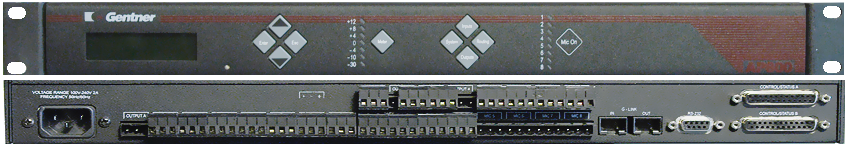
\includegraphics[width=1\textwidth]{images/gentner-ap-800.png}
\caption{Gentner AP-800 echo cancellation device.}
\label{fig:Gentner}
\end{figure}

%%%%%%%%%%%%%%%%%%%%%%%%%%%%%%%%%%%%%%%%%%%%%%%%%%%%%%%%%%%%%%%%%%%%%
%%%%%%%%%%%%%%%%%%%%%%%%%%%%%%%%%%%%%%%%%%%%%%%%%%%%%%%%%%%%%%%%%%%%%
\section{Videoconferencing room}
%%%%%%%%%%%%%%%%%%%%%%%%%%%%%%%%%%%%%%%%%%%%%%%%%%%%%%%%%%%%%%%%%%%%%
%%%%%%%%%%%%%%%%%%%%%%%%%%%%%%%%%%%%%%%%%%%%%%%%%%%%%%%%%%%%%%%%%%%%%

The room we chose for AccessGrid had originally served as an office for the organisation. We therefore had to work within certain constraints, since its original function had to be preserved. Our approach demonstrates that other organisations can follow a similar path at minimal cost. The main changes were:
\begin{paklist}
%-----------------------
\item Preparing projection surfaces by using two walls, which had to be repainted with a fresh coat of white paint.
%-----------------------
\item Installing loudspeakers in the corners of the room.
%-----------------------
\item Installing additional spotlights in one corner of the room.
%-----------------------
\item Installing a cabling system consisting of VGA (computer--projector), S-Video (camera--computer), STP (computer--switch) and audio (microphone--mixer, amplifier--speakers) connections.
\end{paklist}

\begin{figure}
\centering
\includesvg[width=1\textwidth]{arch-ciant-ag-room}
\caption{Room used for videoconferencing.}
\label{fig:CIANT-AG-room}
\end{figure}

Figure \ref{fig:CIANT-AG-room}(A) shows the layout of objects in the room. For video projection, we used two white walls (6a, 6b). Projection is provided by three projectors (5a, 5b), as shown in Figure \ref{fig:CIANT-AG-room}(C), connected to the AG-Display computer (8). The microphone (2) is positioned at the front of the room. It captures sound over a sufficiently wide angle, as also shown in Figure \ref{fig:CIANT-AG-room}(D), together with the arrangement of the loudspeakers (7a, 7b, 7c) in the corners of the room. Microphone audio is sent through the audio mixer (3) directly to the AG-AudioVideo computer (8). Correct operation of the echo-cancellation device (Gentner AP-800) is essential. Figure \ref{fig:CIANT-AG-room}(D) makes it clear that the microphone captures a substantial amount of sound from the loudspeakers, which would otherwise cause unpleasant echo at all connected nodes.

Because of its limited size, the room can accommodate no more than 15 people. This has not yet proved to be a problem, since we have not reached that number. Participants are divided into two categories: active and passive. Active participants sit at the front of the room, around the microphone (2). The moderator sits at position (1). This also determines the arrangement of the cameras (4a, 4b), shown in Figure \ref{fig:CIANT-AG-room}(B). The main camera (4a) captures the moderator and the people closest to them. The secondary camera (4b) captures most of the audience. The operator sits at position (8) and is responsible for the technical operation of the conference. In case of problems, the operator communicates with the other operators using text messages.

%%%%%%%%%%%%%%%%%%%%%%%%%%%%%%%%%%%%%%%%%%%%%%%%%%%%%%%%%%%%%%%%%%%%%
%%%%%%%%%%%%%%%%%%%%%%%%%%%%%%%%%%%%%%%%%%%%%%%%%%%%%%%%%%%%%%%%%%%%%
\section{Day-to-day operational experience}\label{kap:CiantSkusenosti}
%%%%%%%%%%%%%%%%%%%%%%%%%%%%%%%%%%%%%%%%%%%%%%%%%%%%%%%%%%%%%%%%%%%%%
%%%%%%%%%%%%%%%%%%%%%%%%%%%%%%%%%%%%%%%%%%%%%%%%%%%%%%%%%%%%%%%%%%%%%

Originally, we planned to use three projectors. The two main projectors were intended to display video from the VIC application, while the third would display the AG-Display computer's controls and shared presentations.
After several conferences, however, we found that two projectors were sufficient. Moreover, the recording method we used at the time could capture the image from only one projector.

Despite their simplicity and limitations, our first attempts at recording conferences proved very useful. The results can be viewed on the project's wiki pages \cite{CIANT-AGnodeWiki}, including recordings of the Polylogues conferences mentioned above \cite{CIANT-Polylogues-1}, \cite{CIANT-Polylogues-2} and \cite{CIANT-Polylogues-3}.

Recording worked by using the graphics card's ability to clone the image from one VGA output to an S-Video output. We connected this signal to a digital video camera and recorded it onto Mini-DV tapes. After the conference, we digitised the recording into an FLV or MPEG file.

The main advantages of this solution are its simplicity and the fact that it does not interfere with the conference at the software level. We do not need to process the RTP packet stream, and problems caused by increased latency and jitter are avoided. The result is a Mini-DV tape, which also serves as a suitable backup medium.

There are several disadvantages, however. The image from the graphics card, delivered as an S-Video signal, has a maximum resolution of 1024x768. This resolution is already hardware-scaled to 800x600, so the recorded image is slightly lower in quality than the original image displayed on the projection screen.
The resulting recording does not take full advantage of AccessGrid technology. Furthermore, this method can record the image from only one projector. We addressed this limitation by simply not using the additional projectors, or by displaying less important content on them. In that case, the conference operator must decide which video signals and shared presentations are most important. This increases the operator's cognitive load: in addition to managing the technical operation, they must also pay attention to the content of the conference. This can be particularly demanding when the conference deals with a subject that is unfamiliar to the operator.

Another disadvantage is the need to convert the Mini-DV format to MPEG afterwards. This solution also does not allow stored data streams to be played directly in a new conference. All elements are mixed into a single audio-video recording, just as participants saw them through the projection system.

As mentioned above, our room can accommodate 15 people. In such a crowded space, adequate ventilation is necessary, but our solution essentially ignores this requirement. Ventilation is handled in a simple way by opening a window. During our first transmissions, however, we encountered a problem: noise and light from outside disturbed the sensitive conditions inside the room. Opening the window was therefore not an option, and participants had to endure uncomfortable heat and stale air.

Room lighting is another important factor. On the one hand, a dark environment is desirable for projection. On the other hand, the cameras need sufficient light to capture the participants. We resolved this conflict in favour of better lighting. A dark environment not only reduces image quality and makes participants sleepy, but also increases the video bitrate. In poor lighting conditions, the camera introduces random image artefacts that make the image more difficult to encode.

When installing the cabling, we had to ensure that the individual components were properly shielded. We found that running VGA cables alongside power and S-Video cables could cause interference and distort the image.
\proofed
